\documentclass[
  coursecode={APSC 171},
  assignmentname={Week 9 Material Tutorial Solutions},
  solutiontitle=Solution,
  nodate,
  draft,
  % final,
]{
  ltxanswer%
}

\usepackage{bch-style}

\begin{document}
  \begin{questions}
    \setcounter{question}{35}
    \question{}
    \begin{solution}
      \begin{answerfigure}
        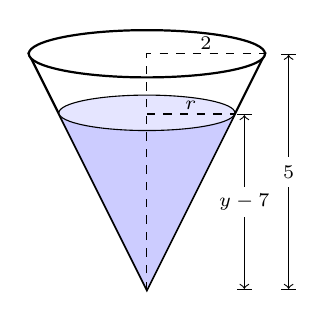
\begin{tikzpicture}[scale=0.75,important line/.style={thick}]
          \draw [opacity=1,important line] (-2,4) -- (2,4) -- (0,0) -- cycle;%big triangle
          \draw [important line,fill=white,opacity=1] (0,4) circle (2cm and 0.4cm);%top of cone
          \draw [fill=blue!20!white,opacity=1] (-1.49,2.98) -- (1.49,2.98) -- (0,0) -- cycle;%smmall triangle
          \draw [fill=blue!10!white,opacity=1,] (0,3) circle (1.49cm and 0.3cm); %top of small cone
          \draw[dashed] (0,0) -- (0,4) --(2,4); %dashed lines
          \draw (1,4.18) node{\scriptsize\(2\)}; % number
          \draw[dashed] (0,2.98) -- (1.49,2.98); %dashed line
          \draw (0.745,3.12) node{\scriptsize\(r\)}; % r
          \draw[|<->|] (2.4,0) -- (2.4,4); %lenght indicator
          \draw[white, fill=white] (2.3,1.75) rectangle (2.5,2.25); %an empty box for the space in middle
          \draw (2.4,2) node{\scriptsize\(5\)}; %a number
          \draw[|<->|] (1.65,0) -- (1.65,2.98); %lenght indicator
          \draw[white, fill=white] (1.45,1.24) rectangle (1.65,1.74);%white rectangle for a space in middle
          \draw (1.65,1.49) node{\scriptsize\(y-7\)};
        \end{tikzpicture}
        \caption{Diagram of the conical portion of the water tank}
        \label{fig:conical-diagram}
      \end{answerfigure}
      Let \(y\) denote the height of any given ``drop'' of water in the tank, where \(y={\qty{0}{\m}}\) \textit{is the base of the tank} and \(y=5+7=\qty{12}{\m}\) is the top of the tank. Then \(y-7\) for \(y \in [7,12]\) represents the height of water in the conical portion of the tank.

      Let \(W_{S}(y)\) denote the total amount of work done by letting a slice water of thickness \(\Delta y\) in the tank at height \(y\) drain and let \(W_{T}\) be the integral we want to construct. Then
      \begin{align*}
        W_{S}(y)             &= F \cdot d                                                \\
                             &= (m g) (y)                                                \\
                             &= (\rho V) g y                                             \\
                             &= \rho (\pi r^{2} \Delta y) g y                            \\
        \intertext{From Figure~\ref{fig:conical-diagram}, we can represent a water slice's radius using similar triangles:}
        \frac{r}{y-7}        &= \frac{2}{5}                                              \\
        r                    &= \frac{2}{5} (y-7)                                        \\
        \Rightarrow W_{S}(y) &= \rho \pi \biggl(\frac{2}{5}(y-7)\biggr)^{2} g y \Delta y \\
                             &= \frac{4}{25} \rho g \pi y (y-7)^{2} \Delta y             \\
                             &= 1568 \pi y(y - 7)^{2} \Delta y
        \intertext{\(\therefore\) the total amount of work done can be represented as}
        W_{T}                &= \sum W_{S}(y)                                            \\
        \alignedbox{         &= 1568 \pi \int_{9}^{12} y(y - 7)^{2} \dl3y}
      \end{align*}
      \begin{note}
        If we defined \(y\) differently, then the integrand (\(d\) and \(r\) as functions of \(y\)) and the bounds of the integral would change. But the overall value of the integral would remain unchanged.
      \end{note}
    \end{solution}

    \question{}
    \begin{solution}
      The integrand is a rational function that can undergo partial fraction decomposition to simplify the evaluation of the integral, since \(\deg(4x-2) < \deg(x^{2}-2x+1)\).\ i.e., the integrand is a proper rational function.

      Let \(I\) denote the value of the indefinite integral. Then using partial fraction decomposition yields
      \begin{align*}
        I                                  &= \int \frac{4x-2}{x^{2}-2x+1} \dl3{x}                       \\
                                           &= 2 \int \frac{2x-1}{(x-1)^{2}} \dl3{x}                      \\
                                           &= 2 \int \frac{c_{1}}{x-1} + \frac{c_{2}}{(x-1)^{2}} \dl3{x} \\
        \Rightarrow \frac{2x-1}{(x-1)^{2}} &= \frac{c_{1}}{x-1} + \frac{c_{2}}{(x-1)^{2}}                \\
        2x-1                               &= c_{1}(x-1) + c_{2}\numberthis\label{eq:constants}          \\
        2x-1                               &= c_{1}x - c_{1} + c_{2}                                     \\
        \Rightarrow                        &\begin{cases}
                                              2x = c_{1}x \\
                                              -1 = -c_{1} + c_{2}
                                            \end{cases}                                           \\
        \Rightarrow                        &\begin{cases}
                                              c_{1} = 2 \\
                                              c_{2} = 1
                                            \end{cases}
        \intertext{\begin{note}
                       The constants can also be solved for by substituting in certain values of \(x\) into~\eqref{eq:constants}.
                     \end{note}}
        \Rightarrow I                      &= 2 \int \frac{2}{x-1} + \frac{1}{(x-1)^{2}} \dl3{x}         \\
        \alignedbox{                       &= 2(2\ln\abs{x-1} - (x-1)^{-1}) + C}.
      \end{align*}
    \end{solution}
  \end{questions}
\end{document}
